Como la mayoría de las aplicaciones DAW modernas, Traverso emplea un esquema jerárquico de enrutación (\FigB~\ref{fig_routing01}), enviando la señal de audio desde los Clips de Audio a las Pistas, desde las Pistas al Master Bus, y después al driver de audio o al sistema operativo. Este esquema no sólo agrupa cosas que son de la misma categoría, también permite aplicar efectos donde sea más eficiente desde el punto de vista de la usabilidad y de la carga del sistema. 

\begin{figure}[t]
 \centering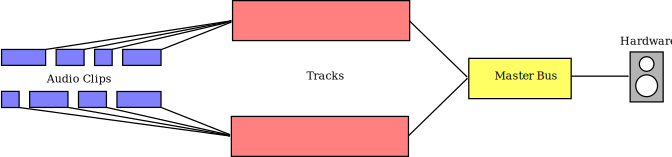
\includegraphics[width=\textwidth]{../images/routing1}
 \caption{En una disposición típica de enrutamiento, la señal es leída por los Clips de Audio (de un fichero en disco), envíada a la pista, y al master bus. Cada nivel aplica su procesado (ganancia, efectos) antes de enviar la señal al nivel siguiente.}
 \label{fig_routing01}
\end{figure}

\section{Trabajar con Clips de Audio}
Los Clips de Audio están en el nivel más bajo de la jerarquía del enrutamiento. Representan archivos de audio leídos desde el disco duro. Los Clips de Audio siempre están en una Pista. Su función principal es establecer \emph{qué} se reproduce y \emph{dónde} se reproduce.

Se crea un clip de audio cuando se importa un archivo de audio (\sact{I}). Puede crearse un clip vacío pulsando \sact{I O} (insertar silencio), pero no se pueden cargar datos en ese clip una vez ha sido creado. Para borrar un clip, haga \dact{R}. Los clips pueden ser movidos libremente con \hact{D} y moviendo el ratón. Si el símbolo de bloqueo aparece enmedio del clip, éste está protegido contra movimientos accidentales. Use \sact{L} para bloquear/desbloquear clips de audio. Si el modo pegajoso está activo, (\sact{SN}), los dos extremos del clip movido intentarán coincidir con el principio de la hoja, con bordes de otros clips, con marcadores, y con el cursor de trabajo. Si quiere mover más de un clip a la vez, use alguna de las funciones siguientes:

\begin{description}
  \item[Selección:] Pueden seleccionarse varios clips pulsando \sact{S}. Acciones de desplazamiento \hact{D} aplicadas a un clip de la selección, se aplicarán a todos. Use \sact{A S} para seleccionar un clip y deseleccionar los demás, y \dact{S} para seleccionar todos los clips de la hoja, o para deseleccionar los que haya seleccionados. Use \sact{S D} para quitar un clip de la selección.
  \item[Encarpetar Pista:] El uso de la función Encarpetar Pista (CTRL $+$ \hact{D F}) desplaza todos los clips de la pista que estén en la posición del cursor o posterior. Esta función se usa por ejemplo cuando se quiere crear un espacio en una pista, sin cambiar la posición relativa de los clips siguientes al espacio.
  \item[Encarpetar Hoja:] Es parecido a Encarpetar Pista. La acción de Encarpetar Hoja (\hact{D F}) mueve todos los clips de la hoja que estén en la posición del cursor o posterior, sin importar en qué pista estén. Esta función se puede usar para mantener la sincronización entre pistas de los clips que se están moviendo.
\end{description}

Todas las acciones presentadas anteriormente se usan para posicionar el clip de audio, es decir, \emph{dónde} se va a reproducir. Para establecer \emph{qué} se va a reproducir, o qué parte de un clip, existen las funciones recortar y dividir. Mueva el ratón sobre un clip, mantenga \hact{E}, y mueva el ratón horizontalmente para ajustar el borde del clip que esté mas cercano a la posición del ratón. Si el modo pegajoso está activo, el borde intentará ajustarse a las posiciones que se mencionaron anteriormente. Los clips pueden ser divididos posicionando en ratón en la posición deseada y pulsando \sact{X}. Por supuesto los bordes de los dos fragmentos pueden ajustarse en detalle usando \hact{E} como se expuso antes. Además del posicionado de los bordes del clip, su comienzo y final pueden regularse usando fades y curvas de ganancia.

\subsection{Fades}
Puede hacerse fade en ambos extremos de un clip, haciendo \hact{F} en la mitad derecha o izquierda del clip y moviendo el ratón horizontalmente. En la mitad izquierda se creará un fade de entrada, y en la mitad derecha un fade de salida. Están disponibles varias formas de fade, que pueden intercambiarse pulsando \sact{M} en la región del fade (\FigB~\ref{fig_fades01}).

\begin{figure}[t]
 \centering\includegraphics[width=0.8\textwidth]{../images/fades}
 \caption{En Traverso están disponibles varias formas de fade. Las curvas empleadas son splines con dos puntos de control (círculos), que pueden modificarse a través de los valores de ``inclinación'' y de ``intensidad''}
 \label{fig_fades01}
\end{figure}

Todas las formas están basadas en un spline cúbico con cuatro parámetros. Dos parámetros definen la inclinación de las curvas no lineales. Con la posición de los puntos de control, se modifica la ``inclinación'' y la ``intensidad''. La ``inclinación'' define la dirección de la tangente en ese extremo, y la ``intensidad'' define el peso de la tangente (\FigB~\ref{fig_fades02}). Los puntos de control no se pueden mover libre e independientemente. En lugar de ello, Traverso implementa varios modos que son apropiados para dar forma a un fade (\FigB~\ref{fig_fades01}):

\begin{figure}[t]
 \centering\includegraphics[width=0.8\textwidth]{../images/fades2}
 \caption{Los valores de inclinación e intensidad se usan para cambiar la forma de las curvas de fade (se muestra con el modo ``Largo'').}
 \label{fig_fades02}
\end{figure}

\subsubsection{Lineal}
Los fades lineales consisten en una línea recta entre el punto inicial y final. Los puntos de control no se pueden cambiar. Los fades lineales tienden a resultar bruscos en el entorno del punto de volumen nulo. Por ello es preferible no usarlos para fades largos de salida (por ej. al final de una hoja).

\subsubsection{Forma de S}
La forma de S empieza con pendiente horizontal, es muy inclinada en el centro, y termina también con pendiente horizontal. El comienzo y el final son muy suaves, pero la parte central puede ser demasiado abrupta en fades cortos. Puede usarse el parámetro de ``intensidad'' para suavizar la parte central y hacer menos notoria la variación de volumen. El parámetro de inclinación debe en general conservarse, aunque puede usarse tangente vertical para conseguir efectos.

\subsubsection{Inclinada}
El modo inclinado es parecido al de forma de S, pero con los puntos de control hacia el mismo lado. Este modo puede usarse para conseguir cambios de volumen muy rápidos al principio del fade de salida, y muy suaves al final. Los dos parámetros de control son útiles para encontrar el equilibrio entre un comienzo no demasiado rápido, y un final que aún se oiga entre los otros clips que existan. 

\subsubsection{Largo}
El modo largo permite ajustar solamente el extremo de volumen nulo del fade. Este modo se suele usar para fades de salida muy largos y progresivos. En el extremo de volumen nominal el cambio es rápido, pero la cola de salida es muy larga. Suele sonar más musical que un modo inclinado equivalente. 

Es posible editar los valores numéricos del fade pulsando \sact{E} en un clip, y yendo a la página ``Fades'' de la ventana de ajustes del clip.

\subsection{Curva de ganancia}
Las curvas de ganancia son una herramienta potente para cambiar la ganancia de un clip de audio a lo largo de la línea de tiempo. Las curvas son elementos hijos de los clips de audio, por tanto su posición \emph{relativa} respecto del clip se mantendrá. Para ver las curvas hay que habilitar el ``Modo: Efectos'', que se puede seleccionar en el menú superior (\FigB~\ref{fig_gcurve01}). Para volver al modo edición, seleccionar ``Modo: Editar''. Existe desde el principio una curva de ganancia por defecto, a 0~dB. Pueden crearse nodos nuevos en la posición del cursor, haciendo \dact{C}. Los nodos pueden ser movidos (\hact{D}) y borrados (\dact{R}). Estas acciones siempre se aplican al nodo más cercano al ratón, el cual se resalta mediante un color diferente.

\begin{figure}[t]
 \centering\includegraphics[width=\textwidth]{../images/gcurve01}
 \caption{El ``modo efectos'' puede activarse desde el menú superior. Las curvas de ganancia sólo son visibles en este modo. Los nodos pueden moverse, añadirse, y borrarse libremente.}
 \label{fig_gcurve01}
\end{figure}

\section{Trabajar con Pistas}
Las pistas reciben la señal de audio de sus clips hijos. Puede añadirse una pista nueva pulsando \dact{T}. Para quitar una pista pulse \dact{R}. Todos los clips de audio que estuvieran en la pista, también serán borrados.

Mientras que los clips representan archivos de audio o ``tomas'', las pistas representan canales completos, o instrumentos. Por tanto se recomienda aplicar en las pistas los efectos que afecten al instrumento (como ganancia, panorama, o plugins de efectos), y ajustar individualmente un clip sólo cuando sea realmente necesario. Esto mantiene el proyecto ordenado, y reduce la carga del sistema.

Además de tener ganancia, efectos de plugin, y panorama, las pistas pueden ponerse en estado mudo \sact{U} o solo \sact{O} durante el proceso de mezcla. Use las acciones dobles respectivas \dact{} para cambiar el estado de mudo y solo de todas las pistas a la vez.

\section{Plugins}
Traverso admite plugins en formato LV2, que es el sucesor del estándar LADSPA. Los plugins pueden ser añadidos a las pistas pulsando \sact{F5}, lo que abre una lista con todos los plugins LV2 instalados en el sistema (\FigB~\ref{fig_pluglist}). Los plugins activos se mostrarán como campos semitransparentes en la pista. Estos campos tienen su propio menú contextual. Pruebe a colocar sobre ellos el ratón y pulsar \sact{Q} o \sact{Botón derecho del ratón}. Pulsando \sact{E} se abre una ventana genérica que permite ajustar los parámetros del plugin. Puede hacerse que un plugin sea ignorado (\sact{B}, mnemónico de ´´bypass''), o quitarlo (\dact{R}). La versión 0.40.x inserta todos los plugins post-fader. Se dispondrá de soluciones más flexibles en las versiones siguientes.

\begin{figure}[t]
 \centering\includegraphics[width=0.6\textwidth]{../images/plugin-list}
 \caption{Pueden añadirse plugins a una pista pulsando \sact{F5}.}
 \label{fig_pluglist}
\end{figure}


